\documentclass[a4paper]{article}
\usepackage[latin1]{inputenc}
\usepackage[T1]{fontenc}
\usepackage[francais]{babel}
\usepackage{entete}
\usepackage{noitemsep}
\usepackage{euscript} 
\usepackage{amsmath,amssymb,amsfonts,amsthm}
\usepackage{graphicx,graphics,epsfig,subfigure,color}
\usepackage{url}
%\usepackage{algorithm2e}
\usepackage{multicol}
\usepackage{a4wide}
\usepackage{latexsym}
\usepackage{verbatim}
\setlength{\textheight}{23.5cm}
\setlength{\topmargin}{-1cm}
\setlength{\textwidth}{155mm}
\setlength{\oddsidemargin}{2mm}

\usepackage{eurosym}
%\renewcommand{\baselinestretch}{0.85}

%\input{macroAlgo}
%\dontprintsemicolon


\newif\ifcorrection
%\correctiontrue   %% comment for student version

\setlength{\parindent}{0pt}  %%suppression indentation


\begin{document}
\selectlanguage{francais}
\author{D. Fourer, L. Lagon}
\newcommand{\universityname}{IUT d'\'Evry Val d'Essonne}
\newcommand{\deptname}{D\'epartement TC (S3)}
\newcommand{\years}{2023-2024}

%------------------- TITRE -----------------------------------------
\date{Septembre 2023} 
\TDHead{\universityname}{\deptname}{R3.12, RCN3, \years}{\large TD2: (R\'evisions) Fonctions avanc\'ees d'un tableur}
%\TDHead{DUT TC}{}{\large TIC3: Fonctions avanc\'ees d'un tableur}
%-------------------------------------------------------------------


%% Tableau crois\'e dynamique /  Graphique

\exost R\'ecup\'erez le fichier \url{https://fourer.fr/Ens/2324/RCN3/classe.zip} et ouvrez le avec Excel/Libreoffice.
Vous pourrez comparer le r\'esultat avec les valeurs calcul\'ees lors du pr\'ec\'edent TD.
 \ifcorrection
 \textcolor{red}{Il s'agit d'une extraction de la solution du TD1 sans les formules}
 \fi
 \begin{enumerate}
  \item \`A partir du nouveau fichier, cr\'eez un tableau crois\'e dynamique (sur une nouvelle feuille) permettant d'afficher la moyenne des filles (F) et celle 
  des gar\c{c}ons (G) pour chaque mati\`ere dans un tableau. Remarquez vous une diff\'erence significative entre les diff\'erents groupes pour certaines mati\`eres?
 \ifcorrection
 \textcolor{red}{Insert / Pivot Table. Choisir ligne F/G, colo}
 \fi
  \item \`A partir des m\^eme donn\'ees, cr\'eez un graphique en b\^atons permettant de comparer les moyennes des deux groupes (filles/gar\c{c}on) pour chaque mati\`ere.
  \item Fa\^ites la m\^eme chose en fonction de l'\^age (tableaux et graphiques crois\'es dynamiques).
 \end{enumerate}

 %%TODO capture resultat
 
%% Condition / recherche

\exost Dans une entreprise, les commerciaux obtiennent une prime en fonction du r\'esultat
qu'ils ont fait sur l'ann\'ee. Si leur r\'esultat est inf\'erieur \`a une certaine limite (11 500 \euro) dans l'exemple cellule B1),
ils n'ont aucune prime. S'il est sup\'erieur, ils ont une prime correspondant \`a un pourcentage (3,2\%) dans
l'exemple cellule F1) de leur r\'esultat. Par ailleurs, si un commercial n'a pas obtenu de prime mais a pourtant
fait un r\'esultat sup\'erieur \`a une seconde limite (10 500 \euro~dans l'exemple cellule D1), alors il m\'erite d'\^etre 
encourag\'e.

\centering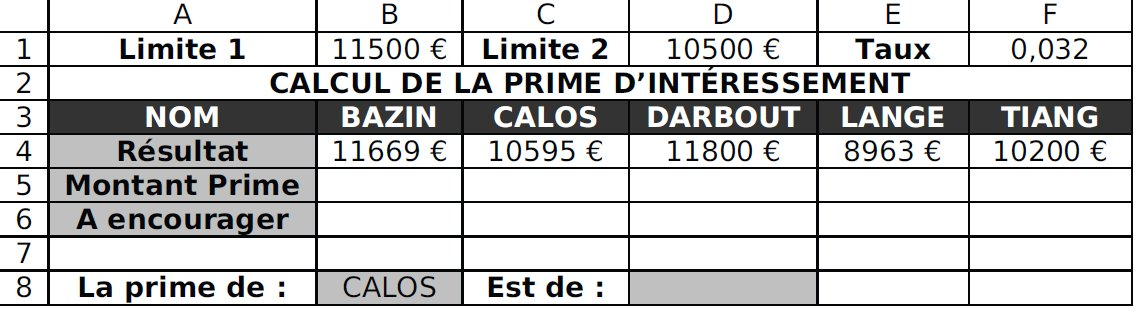
\includegraphics[width=0.7\textwidth]{img/exemple.jpg}

\textbf{Attention:} Les formules que vous utilisez doivent continuer \`a fonctionner si les valeurs des cellules B1, D1, F1 changent.

\begin{enumerate}
 \item Dans la ligne 5 \og{}Montant prime\fg{}, calculez le montant de la prime pour chaque commercial.
 \ifcorrection
 \textcolor{red}{\verb?=IF(B4>B1,0.032*B4)? (fonction SI en Fr)}
 \fi
 \item Dans la ligne 6 \og{}A encourager\fg{}, affichez \og{}oui\fg{} si le commercial se trouve dans ce cas, et rien sinon (rien est une cha\^ine vide " ").
 \ifcorrection
 \textcolor{red}{\verb?=IF(B4<D1,"OUI","")?   }
 \fi
 \item Dans la ligne 8 \og{}La prime de:\fg{}, choisissez le nom d'un commercial de la ligne 3, \'ecrivez le en B8, ajoutez la formule ad\'equate
 dans la cellule D8 pour faire appara\^itre le montant de la prime du commercial choisi. On pourra trouver des fonctions utiles dans la biblioth\`eque \og{}recherche et matrices\fg{}.
 \ifcorrection
 \textcolor{red}{\verb?=HLOOKUP(B7,B3:F5,3)?   (RECHERCHEH en Fr)}
 \fi
 \item Limitez en cellule B8 la saisie du nom \`a la liste des commerciaux (menu donn\'ees, validation).
 \ifcorrection
 \textcolor{red}{data/validity/cell range  (source: B3:F3) }
 \fi
 \item Mettre en forme votre tableau: format de nombre et bordures.
\end{enumerate}


\exost En utilisant la fonction \verb? ALEA() ? qui retourne un nombre al\'eatoire entre 0 et 1, simulez le r\'esultat
d'un nouveau vendeur \og{}SIMULATION\fg{} obtenant un r\'esultat entre 10 000 \euro~ et 15000 \euro ~
(vous trouverez une formule qui retourne toujours un nombre dans cet intervalle).
Assurez vous que votre tableau cr\'e\'e \`a la question pr\'ec\'edente calcule bien sa prime (ou son encouragement).

% (ou RAND() en anglais)


\end{document}

% End Of File

